\clearpage
\section*{Exercise 2: Proteus Schematic}
\addcontentsline{toc}{section}{Exercise 2: Proteus Schematic}

\begin{questionbox}{1. Problem Statement}
Prepare a Proteus circuit for a four-way traffic light with traffic LEDs, four multiplexed seven-segment digits, and three buttons. The connections must match the GPIO definitions in the supplied \texttt{main.h} file.
\end{questionbox}

\vspace{0.4cm}
\textbf{2. Logical Connection Overview}

The following diagram summarizes the logical connections defined by the source code. It is a pin-assignment overview, not an exported screenshot of the complete Proteus schematic.

\begin{figure}[H]
    \centering
    \resizebox{\textwidth}{!}{%
    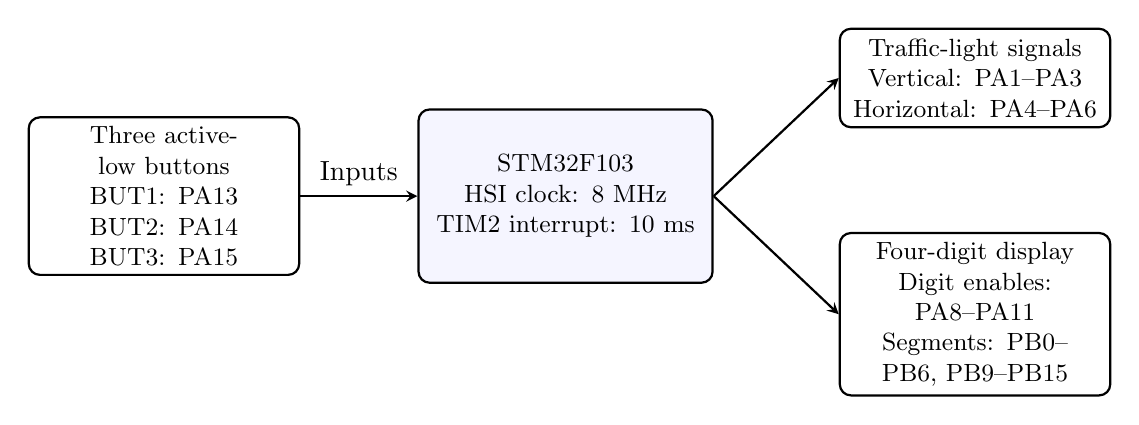
\begin{tikzpicture}[>=stealth, block/.style={draw, rounded corners, align=center, minimum height=1.25cm, text width=3.2cm, font=\small}, controller/.style={draw, rounded corners, align=center, minimum height=2.2cm, text width=3.5cm, fill=blue!4, font=\small}, every path/.style={thick}]
        \node[block] (buttons) at (0,0) {Three active-low buttons\\BUT1: PA13\\BUT2: PA14\\BUT3: PA15};
        \node[controller] (mcu) at (5.1,0) {STM32F103\\HSI clock: 8 MHz\\TIM2 interrupt: 10 ms};
        \node[block] (traffic) at (10.3,1.5) {Traffic-light signals\\Vertical: PA1--PA3\\Horizontal: PA4--PA6};
        \node[block] (display) at (10.3,-1.5) {Four-digit display\\Digit enables: PA8--PA11\\Segments: PB0--PB6, PB9--PB15};
        \draw[->] (buttons.east) -- node[above,draw=none] {Inputs} (mcu.west);
        \draw[->] (mcu.east) -- (traffic.west);
        \draw[->] (mcu.east) -- (display.west);
    \end{tikzpicture}%
    }
    \caption{Logical I/O overview derived from the supplied source files}
    \label{fig:exercise2_logical_io}
\end{figure}

% IMAGE SLOT: Add the screenshot described below and save it as ex02_proteus_complete_schematic.png in the images/ folder.
% If the file is absent, a labeled placeholder is displayed; the document remains compilable.
\begin{figure}[H]
    \centering
    \IfFileExists{images/ex02_proteus_complete_schematic.png}{%
        \includegraphics[width=0.98\textwidth]{images/ex02_proteus_complete_schematic.png}%
    }{%
        \fbox{\parbox[c][5.2cm][c]{0.92\textwidth}{%
            \centering\textbf{IMAGE SLOT -- Full Proteus schematic}\\[6pt]
            Insert a readable full-circuit screenshot showing the STM32, traffic-light LEDs, all four seven-segment digits, three buttons, supply and ground connections, and the wiring between them.\\[6pt]
            \texttt{images/ex02\_proteus\_complete\_schematic.png}%
        }}%
    }
    \caption{Complete Proteus schematic of the traffic-light controller}
    \label{fig:exercise2_full_proteus_schematic}
\end{figure}

\clearpage
\textbf{3. GPIO Pin Assignment}

\begin{table}[H]
    \centering
    \small
    \caption{GPIO assignment defined in \texttt{main.h}}
    \label{tab:exercise2_pinmap}
    \begin{tabularx}{\textwidth}{>{\raggedright\arraybackslash}p{3.0cm} >{\raggedright\arraybackslash}p{2.6cm} X}
        \toprule
        \textbf{Signal} & \textbf{MCU pin} & \textbf{Purpose} \\
        \midrule
        \texttt{R\_1}, \texttt{G\_1}, \texttt{Y\_1} & PA1, PA2, PA3 & Red, green, and amber signals for the vertical road. \\
        \texttt{R\_2}, \texttt{G\_2}, \texttt{Y\_2} & PA4, PA5, PA6 & Red, green, and amber signals for the horizontal road. \\
        \texttt{EN0}, \texttt{EN1} & PA8, PA9 & Vertical display tens and ones digit enables. \\
        \texttt{EN2}, \texttt{EN3} & PA10, PA11 & Horizontal display tens and ones digit enables. \\
        \texttt{SEG1\_0}--\texttt{SEG1\_6} & PB0--PB6 & Seven segment lines for the vertical display. \\
        \texttt{SEG2\_0}--\texttt{SEG2\_6} & PB9--PB15 & Seven segment lines for the horizontal display. \\
        \texttt{BUT1} & PA13 & Select the next mode. \\
        \texttt{BUT2} & PA14 & Increase or decrease a configured timing value. \\
        \texttt{BUT3} & PA15 & Confirm the configured timing value. \\
        \bottomrule
    \end{tabularx}
\end{table}

\begin{figure}[H]
    \centering
    \begin{minipage}[t]{0.48\textwidth}
        \centering
        \includegraphics[width=\linewidth]{images/gpioa_pin_map.png}
        \caption{GPIOA signal labels}
    \end{minipage}\hfill
    \begin{minipage}[t]{0.48\textwidth}
        \centering
        \includegraphics[width=\linewidth]{images/gpiob_pin_map.png}
        \caption{GPIOB segment labels}
    \end{minipage}
    \label{fig:exercise2_pin_evidence}
\end{figure}

\textbf{4. Electrical and GPIO Notes}

The code assumes active-low traffic LEDs, active-low common-anode seven-segment outputs and digit enables, and active-low buttons with pull-ups. It disables SWJ to free PA13--PA15 for GPIO, which affects normal debugging.

The source defines six logical traffic outputs (three colors per road), while the specification asks for 12 physical LEDs (four per color). The Proteus schematic should show how each logical output drives its LED group with suitable current limiting and drivers.
